	Following \citeA{stock&watson1989indexes}, we take data on Industrial Production (IP), total personal income less transfer payments (DPI), total manufacturing and trade sales (TS), and average workweek hours (AW).Note that my data is different from those used by \citeA{stock&watson1989indexes}. I am taking data from 2014-12-15 to 2022-08-31.

% employees on non agricultural payrolls.
	\subsection{Preliminary analysis}
	
	The first step in specifying the model is to test for whether the series are integrated and, if they are, whether they are cointegrated.  As in \citeA{stock&watson1989indexes}, for each of the the coincident indicators, \citeA{dickey1979distribution} test for a unit root (against the alternative that the series are stationary, perhaps around a linear time trend) was unable to reject (at the 10\% level) the hypothesis that the series are integrated. P-values are reported in Table \ref{tab:df_pvalues}.
	
	\begin{table}[h!]
		\centering\small
		\captionsetup{width=0.6\textwidth, font=small}
		\caption{P-values of the test \protect\citeA{dickey1979distribution} for a unit root applied to the four series used in the index estimation. We fail to reject in every case at thte 10\%.}\label{tab:df_pvalues}
		\vspace{0cm}
		\begin{tabular}{l|llll}
			& IP & DPI & TS & AW \\\hline\hline
			p value & 0.08 & 0.33 & 0.98 & 0.47 \\\hline
		\end{tabular}
	\end{table}
 
	The subsequent aplication of the \citeA{engle1987co} test of the nul hypothesis that the four series are not cointegrated against the alternative of cointegration failed to reject at the 10\% significance level. Thus these tests provided no evidence against the hypothesis that each series is integrated but they are not cointegrated. I therefore estimated the model using for the first diference of the logarithm of each of the coincident series, standardized to have zero mean and unit variance.

	\begin{table}[h!]
		\centering\small
		\captionsetup{width=0.6\textwidth, font=small}
		\caption{P-values of the \protect\cite{engle1987co} for cointegration to the four series used in the index estimation. We fail to reject in every case at the 10\% level.}
		\begin{tabular}{l|llll}
		& IP & DPI & TS & AW \\\hline\hline
		IP & - & 0.321725 & 0.174665 & 0.175054 \\
		DPI & 0.814755 & - & 0.091015 & 0.538742 \\
		TS & 0.971659 & 0.139333 & - & 0.731533 \\
		AW & 0.210531 & 0.149117 & 0.026043 & - \\\hline
	\end{tabular}
	\end{table}

\subsection{Maximum Likelihood Estimation}

The parameters of the single-index model have been estimated using IP, DPI, TS and AW over the periods 2006:12-2022:08. As in \citeA{stock&watson1989indexes}, a second order autoregressive  specification  has been adopted for $\Delta C_t$, so that $p=2$. Also, errors $u_t$ are modelled as an $AR(2)$, i.e., $k=2$. The loglikelihood for this model is 274.819. The maximum likelihood estimates of the parameters of the single-index model are presented in Tables  hemaximumlikelihodestimatesoftheparametersofthesingle-index model are presented in Table \ref{tab:ml-params1}

	\begin{table}[h!]
		\centering\small
			\captionsetup{width=0.6\textwidth, font=small}
			\caption{The estimation period is 2006:12-2022:08. The parameters were estimated by Gaussian maximum likelihod as described in the text. The parameters are $\gamma = (\gamma_1,\ldots, \gamma_4)$, $D(L)=\text{diag}\left(d_1(L),\ldots, d_4(L)\right)$, where $d_i(L) = 1-d_{i1}L - d_{12}L^2$ and $\Sigma = \text{diag}\left(1,\sigma_1^2,\ldots,\sigma_4^2\right)$. Maximum likelihood is $\mathcal{L}=274.819$ at the 42688th iteration.}\label{tab:ml-params1}
		\begin{tabular}{l|rrrr}
			& IP & DPI & TS & AW \\\hline\hline
			$\gamma_i$ & 0.592400 & -0.160700 & 0.585400 & 0.320700 \\
			$d_{1i}$ & -0.136700 & -0.277700 & 0.298100 & -0.857200 \\
			$d_{2i}$ & -0.010300 & -0.796800 & -0.288700 & -0.060500 \\
			$\sigma_{i}$ & 0.399400 & 0.611400 & 0.013000 & 0.831200 \\\hline\hline
			&\multicolumn{2}{c}{$\phi_1$} & \multicolumn{2}{c}{$\phi_1$}  \\\hline\hline
			&\multicolumn{2}{c}{0.994600} & \multicolumn{2}{c}{0.639000} \\\hline
		\end{tabular}
	\end{table}

	

	\begin{figure}[h!]
		\centering
		\captionsetup{width=0.6\textwidth, font=small}
		\caption{Evolution of the maximum likelihood, $\mathcal{L}$, during the iteration process. X-axis is plotted in log-scale.}
		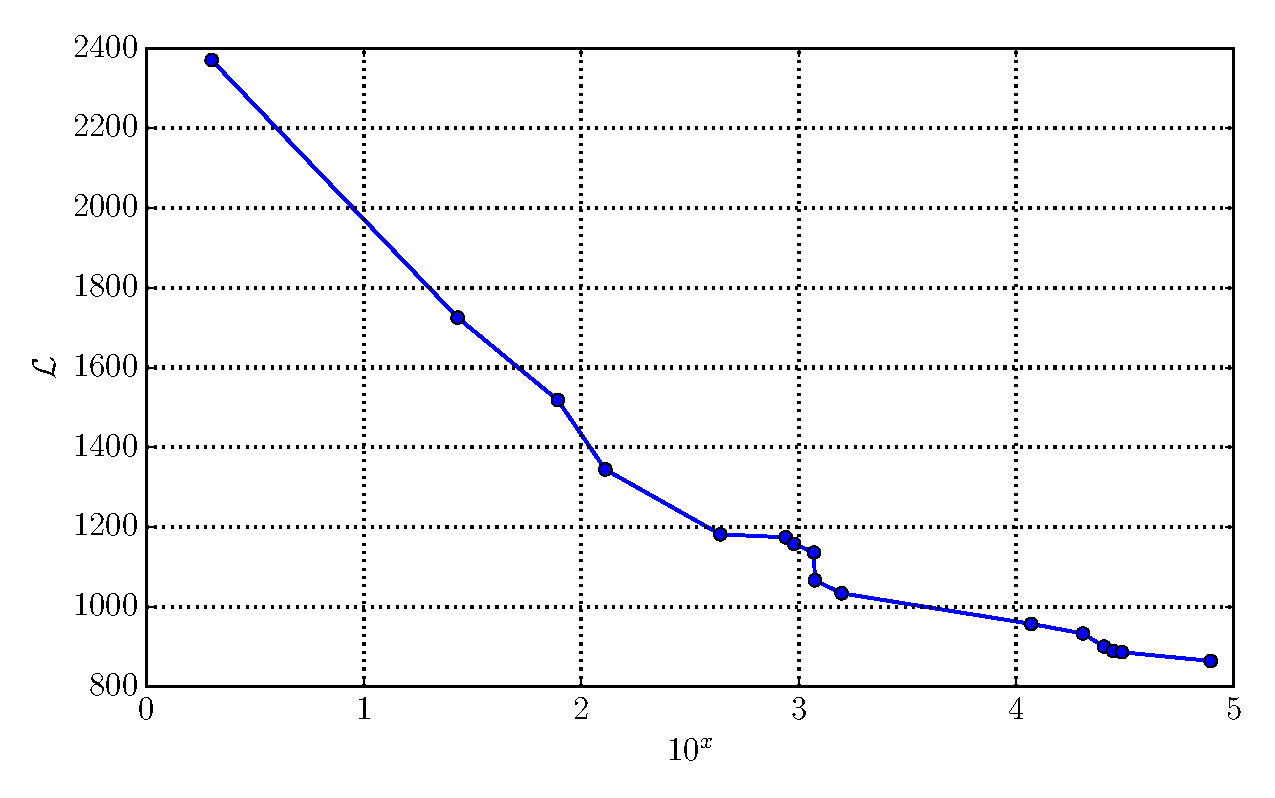
\includegraphics[scale=0.5]{fig/L.eps}
	\end{figure}

		\begin{figure}[h!]
		\centering
		\setlength{\abovecaptionskip}{1pt}
		\captionsetup{width=0.6\textwidth, font=small}
		\caption{$C_{t|t} = \begin{bmatrix}
				Z_c & 0 & 1
			\end{bmatrix} \alpha_{t|t}$.}
		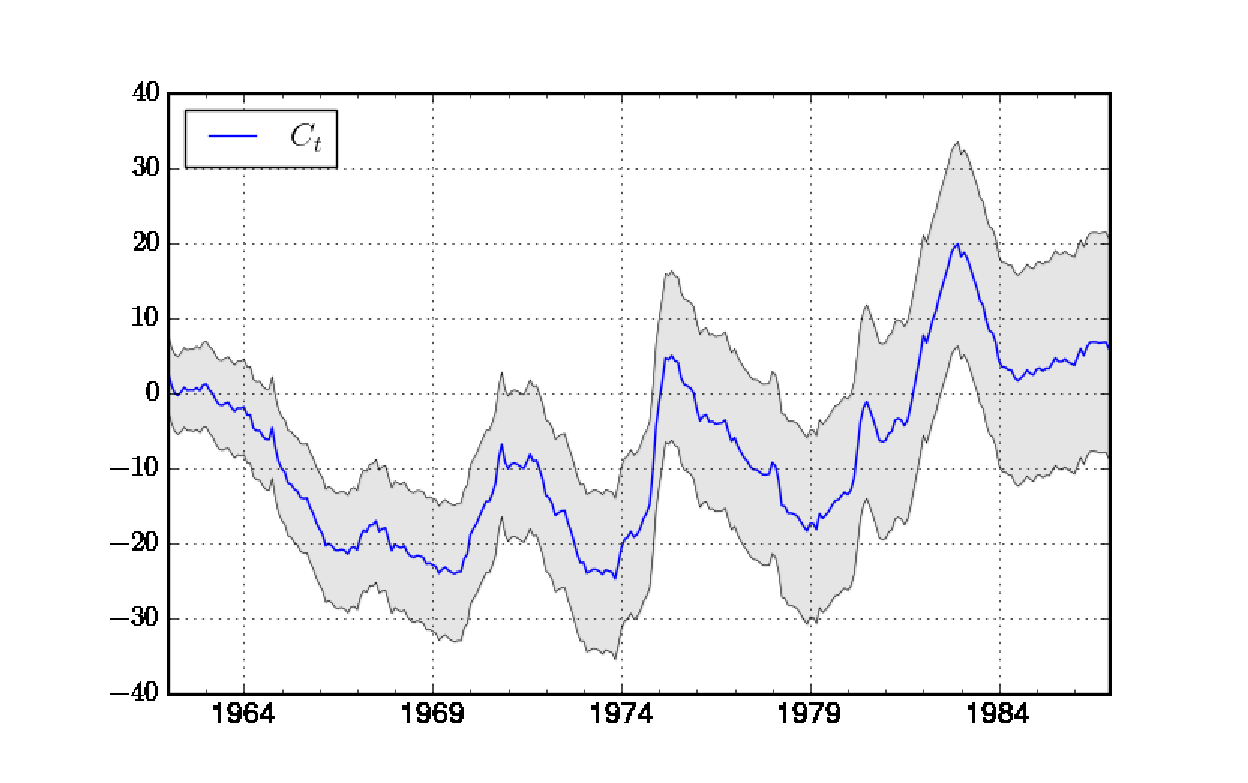
\includegraphics[scale=0.6]{fig/CEI.eps}
	\end{figure}
% IP: aUSIPMANG/CA
% DPI: aUSGPYDPC/CA
% TS: aUSWSLS/A
% AW: USWRKW=ECI
